\documentclass[10pt]{article}

\usepackage[T1]{fontenc}
\usepackage{lmodern}
\usepackage[a4paper,margin=16mm]{geometry}
\usepackage{microtype}
\usepackage{xcolor}
\usepackage{tikz}
\usepackage{pgfplots}
\usepackage{caption}
\usepackage{booktabs}
\usepackage{amsmath}

\usetikzlibrary{arrows.meta,backgrounds,calc,fit,matrix,positioning,shapes.geometric}
\usepgfplotslibrary{groupplots}
\pgfplotsset{compat=1.18}

\definecolor{USTABlue}{HTML}{2563A6}
\definecolor{USTALightBlue}{HTML}{DBEAFE}
\definecolor{USTAGreen}{HTML}{2F855A}
\definecolor{USTALightGreen}{HTML}{DCFCE7}
\definecolor{USTAOrange}{HTML}{D97706}
\definecolor{USTALightOrange}{HTML}{FFEDD5}
\definecolor{USTAPurple}{HTML}{7C3AED}
\definecolor{USTALightPurple}{HTML}{EDE9FE}
\definecolor{USTASlate}{HTML}{334155}
\definecolor{USTALightSlate}{HTML}{F1F5F9}
\definecolor{USTARed}{HTML}{B91C1C}

\captionsetup{font=small,labelfont=bf}
\setlength{\parindent}{0pt}
\setlength{\parskip}{4pt}
\pagestyle{plain}

\tikzset{
  flow/.style={
    rounded corners=2pt,
    draw=USTASlate,
    line width=.7pt,
    minimum height=12mm,
    text width=22mm,
    align=center,
    font=\small,
    inner sep=2mm
  },
  dataflow/.style={flow,fill=USTALightBlue},
  preprocess/.style={flow,fill=USTALightGreen},
  featureflow/.style={flow,fill=USTALightOrange},
  symbolicflow/.style={flow,fill=USTALightPurple},
  evaluationflow/.style={flow,fill=USTALightSlate},
  arrow/.style={-{Latex[length=2.5mm]},draw=USTASlate,line width=.9pt},
  card/.style={
    rounded corners=2pt,
    draw=USTASlate,
    fill=USTALightSlate,
    line width=.6pt,
    align=center,
    font=\small,
    inner sep=2mm
  }
}

\pgfplotsset{
  every axis/.append style={
    axis line style={draw=USTASlate},
    tick style={draw=USTASlate},
    label style={font=\small},
    tick label style={font=\small},
    title style={font=\bfseries\small},
    grid style={draw=black!12},
  }
}

\pgfplotsset{
  colormap={ustaheat}{
    color(0cm)=(white);
    color(1cm)=(USTABlue)
  }
}

\newcommand{\transitionmatrix}[7]{%
  \begin{scope}[shift={(#2,#3)}]
    \node[font=\bfseries\small,anchor=south] at (1.45,2.95) {#1};
    \node[font=\scriptsize,anchor=e] at (-.08,2.15) {BT00};
    \node[font=\scriptsize,anchor=e] at (-.08,.75) {BT01};
    \node[font=\scriptsize] at (.72,2.65) {BT00};
    \node[font=\scriptsize] at (2.17,2.65) {BT01};
    \pgfmathsetmacro{\ca}{100*#4}
    \pgfmathsetmacro{\cb}{100*#5}
    \pgfmathsetmacro{\cc}{100*#6}
    \pgfmathsetmacro{\cd}{100*#7}
    \filldraw[fill=USTAGreen!\ca!white,draw=white,line width=1pt] (0,1.4) rectangle (1.45,2.55);
    \filldraw[fill=USTAGreen!\cb!white,draw=white,line width=1pt] (1.45,1.4) rectangle (2.9,2.55);
    \filldraw[fill=USTAGreen!\cc!white,draw=white,line width=1pt] (0,0) rectangle (1.45,1.4);
    \filldraw[fill=USTAGreen!\cd!white,draw=white,line width=1pt] (1.45,0) rectangle (2.9,1.4);
    \node[font=\small] at (.725,1.975) {#4};
    \node[font=\small] at (2.175,1.975) {#5};
    \node[font=\small] at (.725,.70) {#6};
    \node[font=\small] at (2.175,.70) {#7};
  \end{scope}%
}

\begin{document}

\begin{center}
  {\LARGE\bfseries LaTeX-Native Paper Figures}\\[3mm]
  {\large Learning a Symbolic Nonverbal Vocabulary from Dyadic Pose and Gaze Interactions}\\[2mm]
  \small All diagrams, plots, labels, and values in this document are rendered directly by LaTeX using TikZ and PGFPlots. No raster image is embedded.
\end{center}
\vspace{5mm}

\begin{figure}[p]
\centering
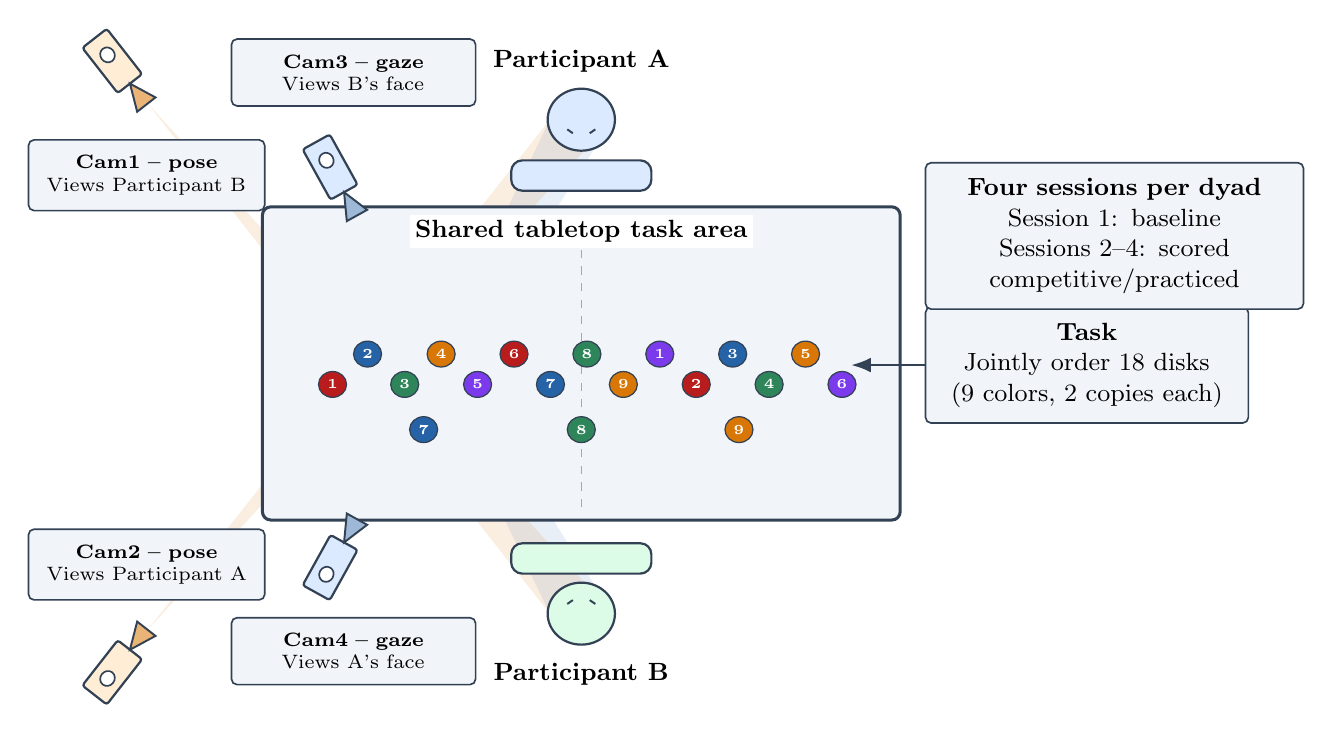
\begin{tikzpicture}[x=.89cm,y=.82cm]
  % Camera fields of view are behind all foreground objects.
  \begin{scope}[on background layer]
    \path[fill=USTAOrange,opacity=.12] (1.79,8.63) -- (7.55,.70) -- (8.45,.70) -- cycle;
    \path[fill=USTABlue,opacity=.10] (4.80,6.92) -- (7.55,.70) -- (8.45,.70) -- cycle;
    \path[fill=USTAOrange,opacity=.12] (1.79,.42) -- (7.55,8.35) -- (8.45,8.35) -- cycle;
    \path[fill=USTABlue,opacity=.10] (4.80,2.11) -- (7.55,8.35) -- (8.45,8.35) -- cycle;
  \end{scope}

  % Table and task objects.
  \draw[rounded corners=3pt,fill=USTALightSlate,draw=USTASlate,line width=1.1pt] (3.45,2.15) rectangle (12.55,7.0);
  \node[font=\bfseries\small,fill=white,inner sep=2pt] at (8,6.62) {Shared tabletop task area};
  \draw[USTASlate!45,dashed] (8,2.35) -- (8,6.35);
  \foreach \x/\y/\c/\n in {
    4.45/4.25/USTARed/1,4.95/4.72/USTABlue/2,5.48/4.25/USTAGreen/3,
    6.00/4.72/USTAOrange/4,6.52/4.25/USTAPurple/5,7.04/4.72/USTARed/6,
    7.56/4.25/USTABlue/7,8.08/4.72/USTAGreen/8,8.60/4.25/USTAOrange/9,
    9.12/4.72/USTAPurple/1,9.64/4.25/USTARed/2,10.16/4.72/USTABlue/3,
    10.68/4.25/USTAGreen/4,11.20/4.72/USTAOrange/5,11.72/4.25/USTAPurple/6,
    5.75/3.55/USTABlue/7,8.00/3.55/USTAGreen/8,10.25/3.55/USTAOrange/9}{
    \filldraw[fill=\c,draw=USTASlate,line width=.45pt] (\x,\y) circle (.20);
    \node[font=\tiny\bfseries,text=white] at (\x,\y) {\n};
  }
  \node[card,text width=37mm,anchor=west] (task) at (12.9,4.55)
    {\textbf{Task}\\Jointly order 18 disks\\(9 colors, 2 copies each)};
  \draw[arrow] (task.west) -- (11.85,4.55);

  % Participant A, facing down toward Participant B.
  \filldraw[fill=USTALightBlue,draw=USTASlate,line width=.8pt] (8,8.35) circle (.48);
  \draw[USTASlate,line width=.7pt] (7.80,8.20) -- (7.88,8.14);
  \draw[USTASlate,line width=.7pt] (8.20,8.20) -- (8.12,8.14);
  \draw[rounded corners=4pt,fill=USTALightBlue,draw=USTASlate,line width=.8pt] (7.0,7.25) rectangle (9.0,7.72);
  \node[font=\bfseries\small,anchor=south] at (8,8.93) {Participant A};

  % Participant B, facing up toward Participant A.
  \filldraw[fill=USTALightGreen,draw=USTASlate,line width=.8pt] (8,.70) circle (.48);
  \draw[USTASlate,line width=.7pt] (7.80,.85) -- (7.88,.91);
  \draw[USTASlate,line width=.7pt] (8.20,.85) -- (8.12,.91);
  \draw[rounded corners=4pt,fill=USTALightGreen,draw=USTASlate,line width=.8pt] (7.0,1.32) rectangle (9.0,1.79);
  \node[font=\bfseries\small,anchor=north] at (8,.08) {Participant B};

  % Camera bodies rotate toward the opposing participant; the triangular lens hood
  % at each camera tip has its point attached to the body and its wide edge facing the viewing direction.
  \begin{scope}[shift={(1.35,9.20)},rotate=-52]
    \draw[rounded corners=1pt,fill=USTALightOrange,draw=USTASlate,line width=.8pt] (-.48,-.24) rectangle (.34,.24);
    \filldraw[fill=USTAOrange!55,draw=USTASlate,line width=.7pt] (.34,0) -- (.72,-.18) -- (.72,.18) -- cycle;
    \filldraw[fill=white,draw=USTASlate,line width=.6pt] (-.18,0) circle (.11);
  \end{scope}
  \node[card,text width=26mm,font=\scriptsize,anchor=north west] at (.10,8.05) {\textbf{Cam1 -- pose}\\Views Participant B};

  \begin{scope}[shift={(4.45,7.55)},rotate=-61]
    \draw[rounded corners=1pt,fill=USTALightBlue,draw=USTASlate,line width=.8pt] (-.48,-.24) rectangle (.34,.24);
    \filldraw[fill=USTABlue!45,draw=USTASlate,line width=.7pt] (.34,0) -- (.72,-.18) -- (.72,.18) -- cycle;
    \filldraw[fill=white,draw=USTASlate,line width=.6pt] (-.18,0) circle (.11);
  \end{scope}
  \node[card,text width=27mm,font=\scriptsize,anchor=south] at (4.75,8.55) {\textbf{Cam3 -- gaze}\\Views B's face};

  \begin{scope}[shift={(1.35,-.15)},rotate=52]
    \draw[rounded corners=1pt,fill=USTALightOrange,draw=USTASlate,line width=.8pt] (-.48,-.24) rectangle (.34,.24);
    \filldraw[fill=USTAOrange!55,draw=USTASlate,line width=.7pt] (.34,0) -- (.72,-.18) -- (.72,.18) -- cycle;
    \filldraw[fill=white,draw=USTASlate,line width=.6pt] (-.18,0) circle (.11);
  \end{scope}
  \node[card,text width=26mm,font=\scriptsize,anchor=south west] at (.10,.90) {\textbf{Cam2 -- pose}\\Views Participant A};

  \begin{scope}[shift={(4.45,1.48)},rotate=61]
    \draw[rounded corners=1pt,fill=USTALightBlue,draw=USTASlate,line width=.8pt] (-.48,-.24) rectangle (.34,.24);
    \filldraw[fill=USTABlue!45,draw=USTASlate,line width=.7pt] (.34,0) -- (.72,-.18) -- (.72,.18) -- cycle;
    \filldraw[fill=white,draw=USTASlate,line width=.6pt] (-.18,0) circle (.11);
  \end{scope}
  \node[card,text width=27mm,font=\scriptsize,anchor=north] at (4.75,.65) {\textbf{Cam4 -- gaze}\\Views A's face};

  \node[card,text width=44mm,anchor=west] at (12.9,6.55)
    {\textbf{Four sessions per dyad}\\Session 1: baseline\\Sessions 2--4: scored competitive/practiced};
\end{tikzpicture}
\caption{Experimental setup and task structure. Each camera icon is oriented toward the opposing participant, and its field-of-view cone terminates at the intended target. Pose cameras target the opposing upper body and face; gaze cameras target the opposing face.}
\label{fig:setup}
\end{figure}
\clearpage

\begin{figure}[p]
\centering
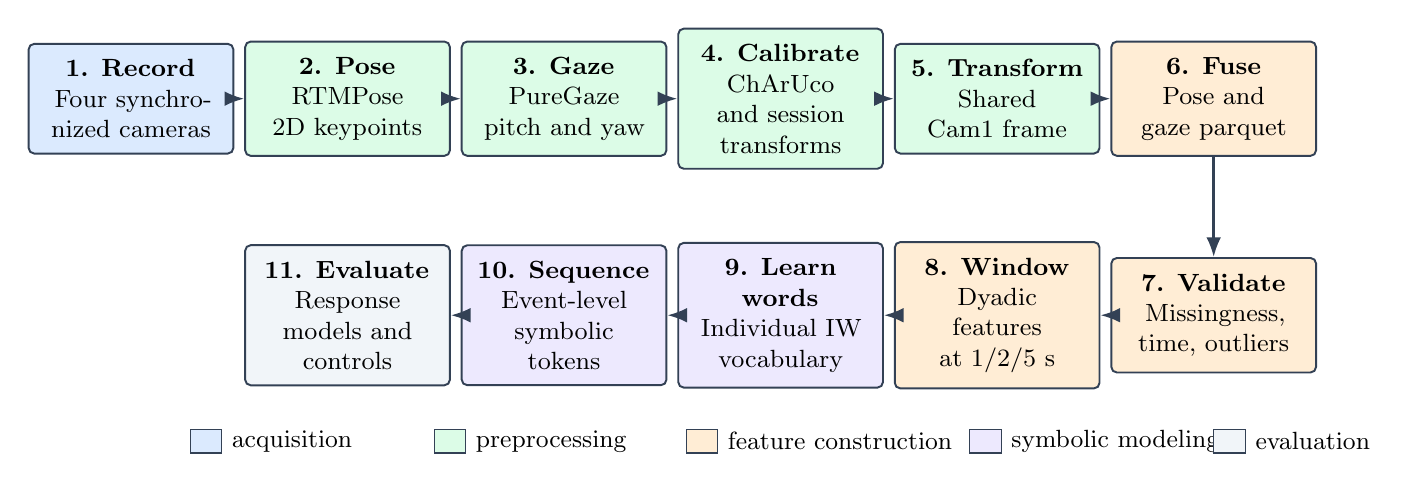
\begin{tikzpicture}[x=1cm,y=1cm]
  % First row: acquisition through fusion.
  \node[dataflow]       (p1) at (1.2,4.3)  {\textbf{1. Record}\\Four synchronized cameras};
  \node[preprocess]     (p2) at (3.95,4.3) {\textbf{2. Pose}\\RTMPose 2D keypoints};
  \node[preprocess]     (p3) at (6.70,4.3) {\textbf{3. Gaze}\\PureGaze pitch and yaw};
  \node[preprocess]     (p4) at (9.45,4.3) {\textbf{4. Calibrate}\\ChArUco and session transforms};
  \node[preprocess]     (p5) at (12.20,4.3){\textbf{5. Transform}\\Shared Cam1 frame};
  \node[featureflow]    (p6) at (14.95,4.3){\textbf{6. Fuse}\\Pose and gaze parquet};

  \draw[arrow] (p1) -- (p2);
  \draw[arrow] (p2) -- (p3);
  \draw[arrow] (p3) -- (p4);
  \draw[arrow] (p4) -- (p5);
  \draw[arrow] (p5) -- (p6);

  % Second row snakes from right to left so text remains large.
  \node[featureflow]    (p7)  at (14.95,1.55) {\textbf{7. Validate}\\Missingness, time, outliers};
  \node[featureflow]    (p8)  at (12.20,1.55) {\textbf{8. Window}\\Dyadic features at 1/2/5 s};
  \node[symbolicflow]   (p9)  at (9.45,1.55)  {\textbf{9. Learn words}\\Individual IW vocabulary};
  \node[symbolicflow]   (p10) at (6.70,1.55)  {\textbf{10. Sequence}\\Event-level symbolic tokens};
  \node[evaluationflow] (p11) at (3.95,1.55)  {\textbf{11. Evaluate}\\Response models and controls};

  \draw[arrow] (p6.south) -- ++(0,-.55) -- (p7.north);
  \draw[arrow] (p7) -- (p8);
  \draw[arrow] (p8) -- (p9);
  \draw[arrow] (p9) -- (p10);
  \draw[arrow] (p10) -- (p11);

  \node[draw=USTASlate,fill=USTALightBlue,minimum width=4mm,minimum height=3mm,label=right:{\small acquisition}] at (2.15,-.05) {};
  \node[draw=USTASlate,fill=USTALightGreen,minimum width=4mm,minimum height=3mm,label=right:{\small preprocessing}] at (5.25,-.05) {};
  \node[draw=USTASlate,fill=USTALightOrange,minimum width=4mm,minimum height=3mm,label=right:{\small feature construction}] at (8.45,-.05) {};
  \node[draw=USTASlate,fill=USTALightPurple,minimum width=4mm,minimum height=3mm,label=right:{\small symbolic modeling}] at (12.05,-.05) {};
  \node[draw=USTASlate,fill=USTALightSlate,minimum width=4mm,minimum height=3mm,label=right:{\small evaluation}] at (15.15,-.05) {};
\end{tikzpicture}
\caption{End-to-end analysis pipeline. The pipeline is arranged in two rows to keep every processing step and arrow readable at paper width.}
\label{fig:pipeline}
\end{figure}
\clearpage

\begin{figure}[p]
\centering
\begin{tikzpicture}
\begin{axis}[
  width=.94\textwidth,
  height=.61\textheight,
  ybar,
  bar width=13pt,
  ymin=0,
  ymax=68,
  ylabel={Prevalence among individual 1 s windows (\%)},
  xlabel={Individual nonverbal word},
  symbolic x coords={IW00,IW01,IW02,IW03,IW04,IW05,IW06,IW07,IW08,IW09,IW10,IW11},
  xtick=data,
  x tick label style={rotate=45,anchor=east},
  ymajorgrids,
  nodes near coords={\pgfmathprintnumber[fixed,precision=1]{\pgfplotspointmeta}\%},
  every node near coord/.append style={font=\scriptsize,rotate=90,anchor=west},
  enlarge x limits=.04,
]
\addplot[fill=USTABlue,draw=USTASlate,line width=.5pt] coordinates {
  (IW00,3.02) (IW01,59.79) (IW02,4.06) (IW03,.86)
  (IW04,3.12) (IW05,1.61) (IW06,6.67) (IW07,5.38)
  (IW08,4.72) (IW09,1.01) (IW10,3.34) (IW11,6.40)
};
\end{axis}
\end{tikzpicture}
\caption{Prevalence of the learned individual nonverbal vocabulary. All bars use one color so magnitude, rather than category color, carries the visual comparison.}
\label{fig:iw-prevalence}
\end{figure}
\clearpage

\begin{figure}[p]
\centering
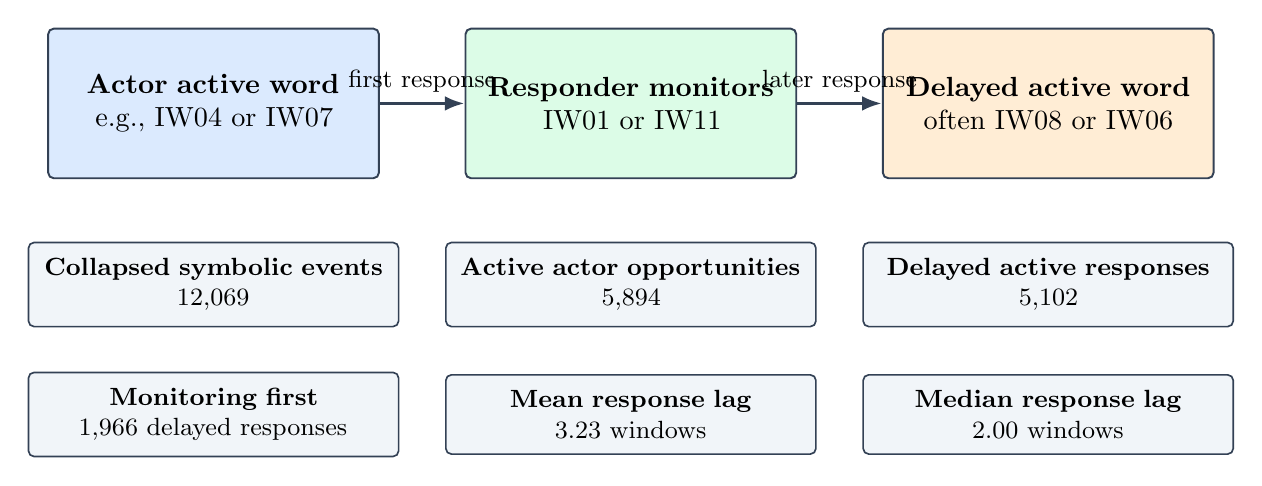
\begin{tikzpicture}[x=1cm,y=1cm]
  \node[flow,fill=USTALightBlue,text width=38mm,minimum height=19mm,font=\normalsize] (a) at (2.7,5.6)
    {\textbf{Actor active word}\\e.g., IW04 or IW07};
  \node[flow,fill=USTALightGreen,text width=38mm,minimum height=19mm,font=\normalsize] (m) at (8.0,5.6)
    {\textbf{Responder monitors}\\IW01 or IW11};
  \node[flow,fill=USTALightOrange,text width=38mm,minimum height=19mm,font=\normalsize] (r) at (13.3,5.6)
    {\textbf{Delayed active word}\\often IW08 or IW06};
  \draw[arrow,line width=1.2pt] (a) -- node[above,font=\small]{first response} (m);
  \draw[arrow,line width=1.2pt] (m) -- node[above,font=\small]{later response} (r);

  \node[card,text width=43mm] at (2.7,3.3) {\textbf{Collapsed symbolic events}\\12,069};
  \node[card,text width=43mm] at (8.0,3.3) {\textbf{Active actor opportunities}\\5,894};
  \node[card,text width=43mm] at (13.3,3.3) {\textbf{Delayed active responses}\\5,102};
  \node[card,text width=43mm] at (2.7,1.65) {\textbf{Monitoring first}\\1,966 delayed responses};
  \node[card,text width=43mm] at (8.0,1.65) {\textbf{Mean response lag}\\3.23 windows};
  \node[card,text width=43mm] at (13.3,1.65) {\textbf{Median response lag}\\2.00 windows};
\end{tikzpicture}
\caption{Event-level symbolic analysis revealed a recurring action--monitoring--action structure.}
\label{fig:event-grammar}
\end{figure}
\clearpage

\begin{figure}[p]
\centering
\begin{tikzpicture}
\begin{axis}[
  width=.94\textwidth,
  height=.60\textheight,
  ybar,
  bar width=17pt,
  ymin=0,
  ymax=1.0,
  ylabel={Score},
  symbolic x coords={Majority,Actor-only,Actor-history,Observed-immediate},
  xtick=data,
  xticklabels={Majority baseline,Actor-only\\Hist-GBDT,Actor-history\\XGBoost,Observed-immediate\\XGBoost},
  x tick label style={align=center,font=\small},
  ymajorgrids,
  legend style={draw=none,at={(.02,.98)},anchor=north west,font=\small},
  nodes near coords={\pgfmathprintnumber[fixed,precision=3]{\pgfplotspointmeta}},
  every node near coord/.append style={font=\scriptsize,anchor=south},
  enlarge x limits=.14,
]
\addplot[fill=USTABlue,draw=USTASlate] coordinates {
  (Majority,.034) (Actor-only,.096) (Actor-history,.429) (Observed-immediate,.779)
};
\addplot[fill=USTAOrange,draw=USTASlate] coordinates {
  (Majority,.523) (Actor-only,.441) (Actor-history,.677) (Observed-immediate,.861)
};
\legend{Macro F1,Top-3 accuracy}
\end{axis}
\end{tikzpicture}
\caption{Event-level response modeling under leave-one-dyad-out evaluation. Observed-immediate models are suitable for offline interpretation because they observe the responder's first post-actor state.}
\label{fig:response-models}
\end{figure}
\clearpage

\begin{figure}[p]
\centering
\begin{tikzpicture}
\begin{axis}[
  width=.90\textwidth,
  height=.58\textheight,
  ybar,
  bar width=14pt,
  ymin=0,
  ymax=1.06,
  ylabel={Score},
  xlabel={Window size},
  symbolic x coords={1s,2s,5s},
  xtick=data,
  xticklabels={1 s windows,2 s windows,5 s windows},
  ymajorgrids,
  legend style={draw=none,at={(.02,.98)},anchor=north west,font=\small},
  nodes near coords={\pgfmathprintnumber[fixed,precision=3]{\pgfplotspointmeta}},
  every node near coord/.append style={font=\scriptsize,rotate=90,anchor=west},
  enlarge x limits=.22,
]
\addplot[fill=USTABlue,draw=USTASlate] coordinates {(1s,.660) (2s,.704) (5s,.768)};
\addplot[fill=USTAOrange,draw=USTASlate] coordinates {(1s,.607) (2s,.659) (5s,.728)};
\addplot[fill=USTAGreen,draw=USTASlate] coordinates {(1s,.924) (2s,.940) (5s,.961)};
\legend{Accuracy,Macro F1,ROC-AUC}
\end{axis}
\end{tikzpicture}
\caption{Pair-identity control experiment. High pair-recognition performance shows that dyads have recognizable signatures and supports leave-one-dyad-out evaluation.}
\label{fig:pair-identity}
\end{figure}
\clearpage

\appendix
\renewcommand{\thefigure}{A\arabic{figure}}
\setcounter{figure}{0}
\begin{figure}[p]
\centering
\begin{tikzpicture}
\begin{axis}[
  width=.72\textwidth,
  height=.73\textheight,
  view={0}{90},
  colormap name=ustaheat,
  colorbar,
  colorbar style={ylabel={Missing ratio},yticklabel style={font=\scriptsize}},
  point meta min=.05,
  point meta max=.46,
  xmin=.5,xmax=4.5,
  ymin=.5,ymax=11.5,
  xtick={1,2,3,4},
  xticklabels={1,2,3,4},
  ytick={1,2,3,4,5,6,7,8,9,10,11},
  yticklabels={dyad\_011,dyad\_010,dyad\_009,dyad\_008,dyad\_007,dyad\_006,dyad\_005,dyad\_004,dyad\_003,dyad\_002,dyad\_001},
  xlabel={Session order},
  ylabel={Dyad},
  nodes near coords={\pgfmathprintnumber[fixed,precision=2]{\pgfplotspointmeta}},
  every node near coord/.append style={font=\scriptsize},
]
\addplot[
  matrix plot*,
  mesh/cols=4,
  point meta=explicit,
] table[meta=value] {
x y value
1 11 .123
2 11 .113
3 11 .131
4 11 .124
1 10 .205
2 10 .168
3 10 .178
4 10 .212
1 9 .288
2 9 .264
3 9 .175
4 9 .201
1 8 .350
2 8 .314
3 8 .149
4 8 .096
1 7 .116
2 7 .096
3 7 .119
4 7 .164
1 6 .098
2 6 .090
3 6 .067
4 6 .131
1 5 .127
2 5 .105
3 5 .110
4 5 .111
1 4 .389
2 4 .222
3 4 .270
4 4 .210
1 3 .388
2 3 .342
3 3 .456
4 3 .410
1 2 .218
2 2 .209
3 2 .230
4 2 .156
1 1 .292
2 1 .122
3 1 .123
4 1 .192
};
\end{axis}
\end{tikzpicture}
\caption{Session-level missingness aggregated by dyad and session order.}
\label{fig:missingness}
\end{figure}
\clearpage

\begin{figure}[p]
\centering
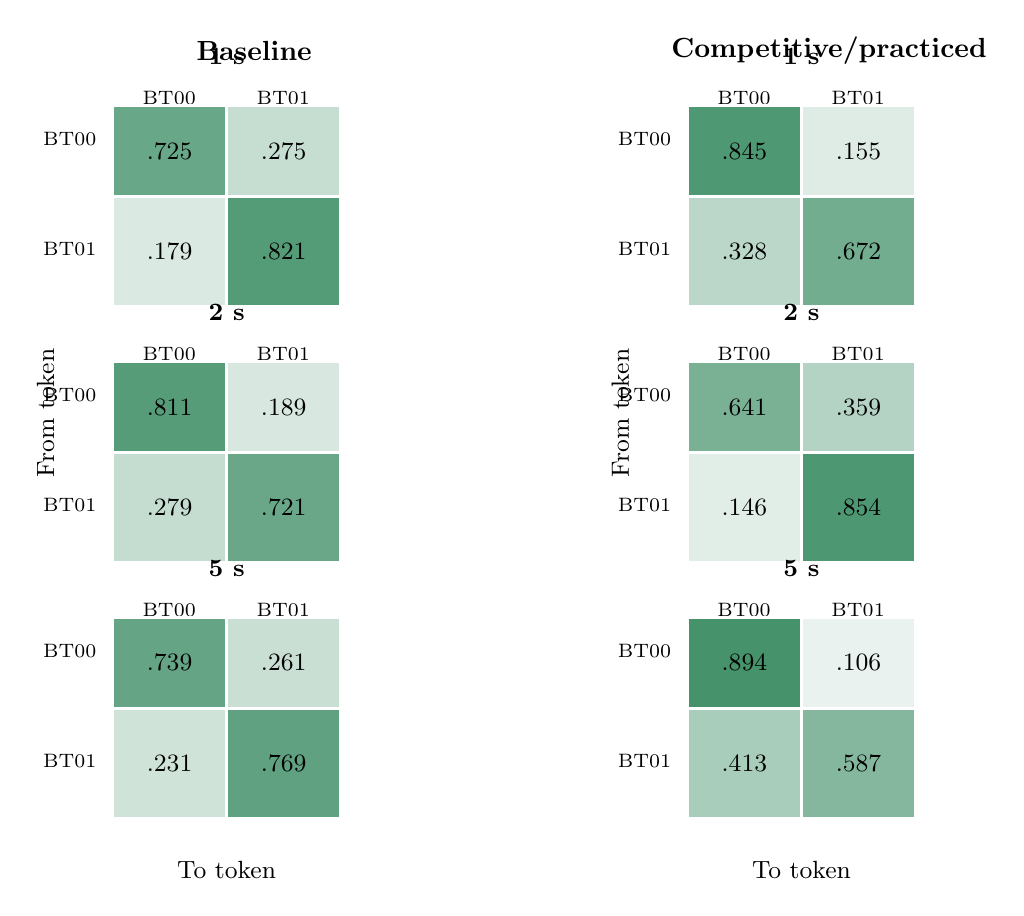
\begin{tikzpicture}[x=1cm,y=1cm]
  \node[font=\bfseries] at (3.0,9.05) {Baseline};
  \node[font=\bfseries] at (10.3,9.05) {Competitive/practiced};
  \transitionmatrix{1 s}{1.2}{5.8}{.725}{.275}{.179}{.821}
  \transitionmatrix{1 s}{8.5}{5.8}{.845}{.155}{.328}{.672}
  \transitionmatrix{2 s}{1.2}{2.55}{.811}{.189}{.279}{.721}
  \transitionmatrix{2 s}{8.5}{2.55}{.641}{.359}{.146}{.854}
  \transitionmatrix{5 s}{1.2}{-.70}{.739}{.261}{.231}{.769}
  \transitionmatrix{5 s}{8.5}{-.70}{.894}{.106}{.413}{.587}
  \node[rotate=90,font=\small] at (.35,4.45) {From token};
  \node[rotate=90,font=\small] at (7.65,4.45) {From token};
  \node[font=\small] at (2.65,-1.35) {To token};
  \node[font=\small] at (9.95,-1.35) {To token};
\end{tikzpicture}
\caption{Baseline and competitive/practiced token transition matrices. Jensen--Shannon divergences are 0.0774 at 1 s, 0.0903 at 2 s, and 0.1081 at 5 s.}
\label{fig:transitions}
\end{figure}
\clearpage

\begin{figure}[p]
\centering
\begin{tikzpicture}
\begin{groupplot}[
  group style={group size=2 by 1,horizontal sep=14mm},
  width=.45\textwidth,
  height=.68\textheight,
  xbar=8pt,
  xmin=0,
  xmax=.70,
  symbolic y coords={Pose 5s,Pose 2s,Pose 1s,Gaze 5s,Gaze 2s,Gaze 1s,Combined 5s,Combined 2s,Combined 1s},
  ytick=data,
  xmajorgrids,
  nodes near coords={\pgfmathprintnumber[fixed,precision=3]{\pgfplotspointmeta}},
  every node near coord/.append style={font=\tiny,anchor=west},
  tick label style={font=\scriptsize},
]
\nextgroupplot[title={Macro F1}]
\addplot[fill=USTABlue,draw=USTASlate] coordinates {
  (.607,{Pose 5s}) (.610,{Pose 2s}) (.621,{Pose 1s})
  (.615,{Gaze 5s}) (.588,{Gaze 2s}) (.579,{Gaze 1s})
  (.614,{Combined 5s}) (.601,{Combined 2s}) (.589,{Combined 1s})
};
\nextgroupplot[title={ROC-AUC},yticklabels={}]
\addplot[fill=USTAGreen,draw=USTASlate] coordinates {
  (.617,{Pose 5s}) (.607,{Pose 2s}) (.613,{Pose 1s})
  (.619,{Gaze 5s}) (.608,{Gaze 2s}) (.600,{Gaze 1s})
  (.619,{Combined 5s}) (.603,{Combined 2s}) (.611,{Combined 1s})
};
\end{groupplot}
\end{tikzpicture}
\caption{Best non-dummy baseline-vs-competitive/practiced random-forest classifier per window size and feature set.}
\label{fig:condition-ablation}
\end{figure}

\end{document}
